\section{Research Method}

%You need to describe briefly the life cycle model or research method that you used. You do not need to write about all of the different process models that you are aware of. Focus on the process model or research method that you have used. It is possible that you needed to adapt an existing method to suit your project; clearly identify what you used and how you adapted it for your needs.

For this project, a literature review was undertaken to assess the work completed by researchers in the fields of Entropy, Fuzzy Entropy and image alignment methods to help better understand what has been investigated, and to gain an understanding of the background.

\subsection{Entropy}
\label{ssec:entropy}

In terms of Information Theory, the Merriam-Webster Dictionary defines Entropy to be \cite{def_entropy}:

\begin{quotation}
 \textit{Entropy (noun): the degree of disorder or uncertainty in a system}
\end{quotation}

Shannon entropy, derived by Claude Shannon \cite{shannon1948a} can be mathematically defined as :

\begin{equation}
  H(X) = - \displaystyle\sum_{i=0}^{N}{p_i \log_2 p_i}
\end{equation}
\myequations{Shannon Entropy}

Where $p_i$ is the set of probabilities for all the variables in $X$.

Let us consider a fair coin toss. The probability of heads is exactly $\frac{1}{2}$, therefore, the entropy of landing on heads is:

\begin{equation}
  \begin{split}
    H(heads) &= -\frac{1}{2}\log_2(\frac{1}{2}) - \frac{1}{2}\log_2(\frac{1}{2}) \\
    &= 1.0
  \end{split}
\end{equation}
\myequations{Shannon Entropy example - coin toss}

On the other side, if a system outputs solely the letter \say{M}, then the entropy of receiving the letter \say{M} is exactly 0. This is because when either the positive or the negative outcome is 100\%, then both sides equal \say{0} when fed into the entropy equation.
%http://mirror.ox.ac.uk/sites/ctan.org/graphics/pgf/contrib/pgfplots/doc/pgfplots.pdf
\begin{figure}[H]
  \iffalse
\begin{center}
\pgfplotsset{every axis/.append style={thick},width=0.4*\textwidth, ymax=1}
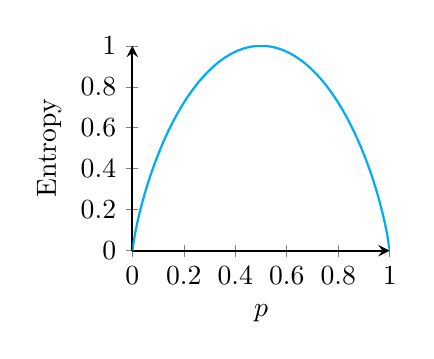
\begin{tikzpicture}
 \begin{axis}[
     axis lines = left,
    xlabel = $p$,
    ylabel = {Entropy},
    ]
  \addplot [
    domain=-0:1,
    samples=100,
    color=cyan,
    ]
    { -( x * log2(x) + (1-x) * log2(1-x) )};
  \end{axis}
\end{tikzpicture}
\end{center}
\caption{Entropy mapped against probability ($p$) of occurrence.}
\label{fig:entropy}
\fi
\end{figure}

It follows that entropy can only ever take a value between 0 and 1, with an entropy of 1 have a 50\% probability, and an entropy of 0 being 100\% certain.

\subsection{Uncertainty}

However real life is not 100\% certain - a small amount of uncertainty in life is to be expected and sometimes desired. A surprise party for many is the nice kind, however uncertainty associated with risk - i.e. \say{Will I lose my job in the recession?} - is uncertainty with a negative impact. Modeling uncertainty is especially important to researchers so they can understand it, and use it to our advantage in techniques such as fuzzy entropy.

\subsubsection{Probabilistic Uncertainty}

By definition:

\begin{quotation}
  \textit{Probability: the chance that something will happen \cite{PROBABILITY}}
\end{quotation}

Probabilistic distribution is a widely accepted and used technique for representing expert judgements of uncertainty \cite{O’Hagan_2011}. Early work carried out by DeGroot (1970) \cite{degroot2004optimal}, built upon that of Savage (1954) \cite{Savage_1954}, gave a simple layman's explanation:

\begin{quotation}
  \textit{For instance, if the person prefers decision A to B and B to C then they must also prefer A to C.}
\end{quotation}

\subsubsection{Possibilistic Uncertainty}

By definition:

\begin{quotation}
  \textit{Possibility: a chance that something might exist, happen, or be true : the state or fact of being possible \cite{POSSIBILITY}}
\end{quotation}

Possibilistic uncertainty (closely related to \say{fuzziness}) indicates the lack of information we hold about the possible outcome values from a system - a sort of ambiguity. Possibilistic uncertainty models the possible outcomes from a system, as estimated by a decision maker because it is possibly impossible to determine beforehand \cite{Untiedt_2010}.

\subsubsection{Indiscernibility Uncertainty}

By definition:

\begin{quotation}
  \textit{Indiscernibility: the quality or state of being indiscernible \cite{INDISCERNIBILITY}}

  \textit{Indiscernible: impossible to see, hear, or know clearly \cite{INDISCERNIBLE}}
\end{quotation}

\todo[inline]{Find an explanation of Indiscernibility}


\subsection{Fuzzy Entropy}
\label{ssec:fuzzy-entropy}

Fuzzy entropy stems from combining standard Shannon entropy with the practices of Fuzzy Set Theory, discovered by Zadeh in 1965 \cite{Zadeh_1965}. This introduces the idea of \say{Membership} to a category, where an object can belong to more than one category to a certain degree.

One common example of this is listing someone as `Short', `Average' or `Tall' in height. If a tall person is someone over 6 feet in height, would a person who measured 5foot 11inches not be classified as tall? Given crisp sets, then they would be classified as `Average'. In fuzzy set theory, they would be be a certain degree of tall, and a certain degree of average, with the highest membership likely to win out when categorising their height. Another example of this can be seen in Figure \ref{fig:fuzzy-sets}

\begin{figure}[H]
  \center
  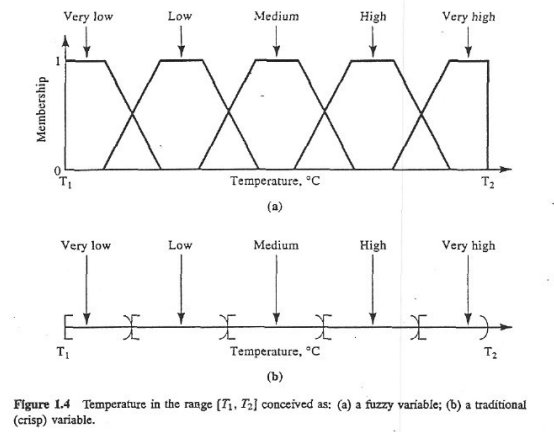
\includegraphics[scale=0.5]{Chapter1/lit-review-img/fuzzy-sets.png}
  \caption{A comparison between Fuzzy Sets and Crisp sets. \textit{Image Source: Fuzzy Sets and Fuzzy Logic: Theory and Applications \cite{GEORGE_J_BO_2008}}}
  \label{fig:fuzzy-sets}
\end{figure}

After combining Fuzzy Set Theory with Entropy, then the amount of fuzzy information gained from the fuzzy set(s) is known as fuzzy entropy.

\subsubsection{Non-Probabilistic Entropy - 1972}
\label{sssec:non-prob-review}

De Luca and Termini are considered to be the first to have taken Shannon Entropy and extended it to include fuzziness \cite{DeLuca_Termini_1972}. They also defined properties which a fuzzy entropy must follow, in order to be classed as true.

Their non-probabilistic fuzzy entropy equation is as given:

\begin{equation}\label{eq:de-luca-eq}
  H_A = -K \displaystyle\sum_{i=1}^{n}{\{\mu_i\log(\mu_i) + (1 - \mu_i)\log(1 - \mu_i)\}}
\end{equation}
\myequations{Non-Probabilistic Entropy}

Where $\mu$ is the maximum membership across all the fuzzy sets.

The entropy given by equation \eqref{eq:de-luca-eq} satisfies all 4 of De Luca and Termini's defined properties:

  \begin{subequations} \label{eq:de-luca-cond}
    \begin{align}
      &\text{\textbf{P-1 }} H_A = 0 \text{ iff } A \text{ is a crisp set (}\mu_i = 0 \text{ o r} 1 \forall x_i \in A\text{)} \\
      &\text{\textbf{P-2 }} H_A \text{ is maximum iff }\mu_i = 0.5 \forall x_i \in A \\
      &\text{\textbf{P-3 }} H \geq H^\ast\text{ where }H^\ast\text{ is the entropy of }A\text{, a sharpened version of } A \\
      &\text{\textbf{P-4 }} H = \overline{H}\text{ where }\overline{H}\text{ is the entropy of the complement set }\overline{A}
    \end{align}
  \end{subequations}


%\subsubsection{Fuzzy entropy and conditioning - 1986}

\subsubsection{Fuzzy Shannon Entropy - 1989}

Sander \cite{Sander_1989} presented a characterisation of a fuzzy entropy some time after De Luca and Termini`s work was published. His implementation of Shannon fuzzy entropy is laid out in equation \eqref{eq:fuzzy-shannon} below:

\begin{equation}\label{eq:fuzzy-shannon}
  H(f) = -c \displaystyle\sum_{i=1}^{n}{f(x_i)lnf(x_i), c > 0}
\end{equation}

Where the power of a fuzzy set is defined as:

\begin{equation}
  P(f) = \displaystyle\sum_{i=1}^{n}{f (x_i)}
\end{equation}

Sander further went on to propose some properties, which must be imposed on a fuzzy entropy $d$ to ensure that $d(f) = H(f)$:

\begin{subequations}
  \begin{align}
    &\text{\textbf{1. Sharpness: }} d(f) = 0 \Leftrightarrow f(X) \subset {0,1}, f \in [0,1]^X \\
    &\text{\textbf{2. Valuation: }} d(f \wedge g) + d(f \vee g) = d(f) + d(g), f,g \in [0,1]^X \\
    \begin{split}
    &\text{\textbf{3. Generalised additivity: }} \text{There exists two mappings s,t: } [0,\infty) \rightarrow  [0,\infty) \\
      &\text{ such that } d(f x g) = d(f)t(P(g)) + s(P(f))d(g) \text{ for all } f \in [0,1]^X, g \in [0,1]^Y, \\
      &\text{ where } X \text{ and } Y \text{ are finite sets.}
    \end{split}
  \end{align}
\end{subequations}

\subsubsection{Object-background segmentation using new definitions of entropy - 1989}

Pal \& Pal outlined their first fuzzy entropy algorithm in 1989 \cite{Pal_Pal_1989}, which satisfies all 4 of De Luca and Termini`s 4 conditions (outlined in Equations\eqref{eq:de-luca-cond}). It as as follows:

\begin{equation} \label{eq:pal-pal-orig}
  H = -k  \displaystyle\sum_{i=1}^{n}{\{\mu_iexp(1 - \mu_i) + (1 - \mu_i)exp(\mu_i)\}}
\end{equation}

\subsubsection{Higher Order Fuzzy Entropy \& Hybrid Entropy - 1992}
\label{sssec:hybrid-section}

In Pal \& Pal's paper \say{Higher order fuzzy entropy and hybrid entropy of a set} \cite{Pal_Pal_1992}, they not only prove some of De Luca \& Termini`s work to be flawed, but also defined two new fuzzy entropy algorithms, and a new set of definitions.

\noindent \textbf{Higher Order Fuzzy Entropy}

As defined by Pal \& Pal:

\begin{itemize}
  \item $P = $ Fuzzy property set
  \item $\mu =$ the degree to which $x_i$ possesses the property $P$
  \item $n =$ number of elements, with $r =$ a combination of elements from group $n$
  \item $S^r_i =$ denotes the $i$th element of such a combination
  \item $\mu(S^r_i) =$ the degree to which the combination $S'$ as a whole possesses $P$
  \item There are $\begin{bmatrix} \bigl(\begin{smallmatrix}
  n \\ r
  \end{smallmatrix} \bigr) \end{bmatrix}$ such combinations
\end{itemize}

The entropy of order $r$ of the fuzzy set $A$ is defined as:

\begin{equation} \label{eq:higher-order}
  H' = \bigg(\frac{I}{\bigl(\begin{smallmatrix}
  n \\ r
\end{smallmatrix} \bigr)}\bigg) \displaystyle\sum_{i=1}^{\bigl(\begin{smallmatrix}
  n \\ r
  \end{smallmatrix} \bigr)} \{ \mu(S^r_i)exp(1 - \mu(S^r_i)) \} + \{ 1 - \mu(S^r_i) \}log\{\mu(S^r_i)\}
\end{equation}

If $r = 1$, then \eqref{eq:higher-order} reduces to Equations \eqref{eq:pal-pal-orig} and \eqref{eq:de-luca-eq}

\noindent \textbf{Hybrid Entropy}

Another fuzzy entropy implementation outlined in Pal \& Pal`s paper was Hybrid Entropy. This algorithm is particularly useful as it combines Probabilistic and Possibilistic (fuzziness) uncertainty and if fuzziness is removed or not present, it returns to that of a classical set.

Let us define Hybrid Entropy.

\begin{itemize}
\item Let $p_0$ and $p_1$ be the probabilities of receiving 0 and 1 symbols over a noisy digital communication line respectively.
\item Let $\mu$ denote the membership functions of the fuzzy set \say{Symbol close to 1}
\item Both $E_1$ is a monotonically increasing function of $\mu$ - $E_0$ can be perceived as the likelihood (possibility) of receiving a \say{1} symbol
\begin{itemize}
    \item as $\mu$ increases from 0 to 1, then $E_1$ also increases
    \item e.g. with an incoming \say{0} symbol, if $\mu$ increases, than the difficulty of correct interpretation also \textit{increases} - a wrong interpretation of a \say{0} becomes likely
    \item e.g. for an incoming \say{1} symbol, if $\mu$ increases, then the difficulty of correct interpretation \textit{decreases} - improving likelihood of correct classification
  \end{itemize}
\item At the same time, $E_0$ can be perceived as the likelihood (possibility) of receiving the \say{0} symbol for the same reasoning
\end{itemize}

$E_0$ and $E_1$ can be defined as:

\begin{subequations} \label{eq:E0-E1}
  \begin{align}
    &E_0 = \frac{1}{n}\displaystyle\sum_{i=1}^{n}{(1-\mu_i)exp(\mu_i)} \\
    &E_1 = \frac{1}{n}\displaystyle\sum_{i=1}^{n}{\mu_iexp(1-\mu_i)}
  \end{align}
\end{subequations}

Therefore, the hybrid entropy of fuzzy set $A$ can be defined as:

\begin{equation}
  H_{hy} = -p_0\log(1 - E_0) - p_1\log(E_1)
\end{equation}

\subsubsection{Fuzzy Entropy: a Brief Survey - 2001}

Due to the older nature of some of the papers listed above, some were difficult to locate online. So when implementing the chosen algorithms (Non-Probalistic Entropy and Hybrid Entropy), Al-sharhan et al's paper \say{Fuzzy Entropy: a Brief Survey} \cite{Al-Sharhan_Karray_Gueaieb_Basir_2001} was a useful tool.

Its concise nature, and chronological listing ensured a strong understanding of the basic principles, before introducing the more complex algorithms (such as Higher Order Fuzzy Entropy). The paper also highlights advantages and flaws to each solution.

\subsection{Joint Image Alignment}

Joint image alignment, occasionally otherwise known as groupwise image alignment, focuses on the alignment of several images, into one average image. This research area has been particularly prevalent in areas such as medical and facial imagery \cite{Tiddeman_Hunter_2011} \cite{Cootes_Twining_Petrovic_Babalola_Taylor_2010}. Cootes et. al. leverage a groupwise registration algorithm to choose one base image with control points to align (typically a standard mesh frame), analyse each following image in turn estimating the movement needed to align corresponding control points, then iteratively warp each image to fit the reference frame, adjusting the texture model as they`re aligned. This type of alignment will not be considered for the project due to the over-complexity needed for the input image, along with computational limitations due to aligning one image at a time with the base image.

This Subsection will look into a couple of the techniques which will be suitable for this project.

\subsubsection{Learned-Miller`s Congealing}

Learned-Miller's \Gls{Congealing} \cite{joint-alignment} is often cited as being one of the first to truly align simple sets of data (which must have minimal noise, no occlusions and illumination variation) \cite{Zhou_Lee_Yu_Efros_2015} \cite{peng2012rasl}. Many more robust image alignment techniques have been developed off of the basis of this work, however with more computational-expense.

This algorithm works by iteratively reducing the pixel-wise entropy over the input images, using a set of standard image transformations, in a \gls{non-deterministic} manner, such as:

\begin{itemize}
  \item $x$ \& $y$ translations (Figure \ref{fig:translation})
  \item rotation (Figure \ref{fig:rotation})
  \item $x$ \& $y$ shear (Figures \ref{fig:x-shear} \& \ref{fig:y-shear} respectively)
  \item $x$ \& $y$ scale (Figure \ref{fig:scale})
\end{itemize}

\begin{center}
  \begin{figure}[H]
      \begin{subfigure}[b]{0.45\textwidth}
        \centering
            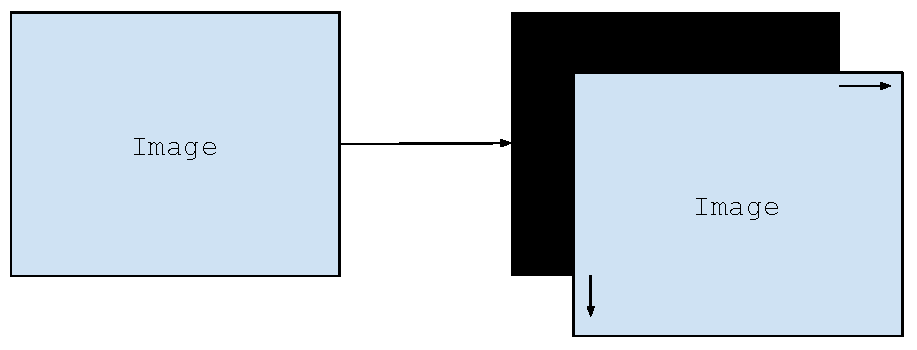
\includegraphics[width=\textwidth]{Chapter1/lit-review-img/translation.pdf}
          \caption{Image translation in the $x$ \& $y$ axes.}
          \label{fig:translation}
      \end{subfigure} \hfill
      ~ %add desired spacing between images, e. g. ~, \quad, \qquad, \hfill etc.
        %(or a blank line to force the subfigure onto a new line)
      \begin{subfigure}[b]{0.45\textwidth}
          \centering
          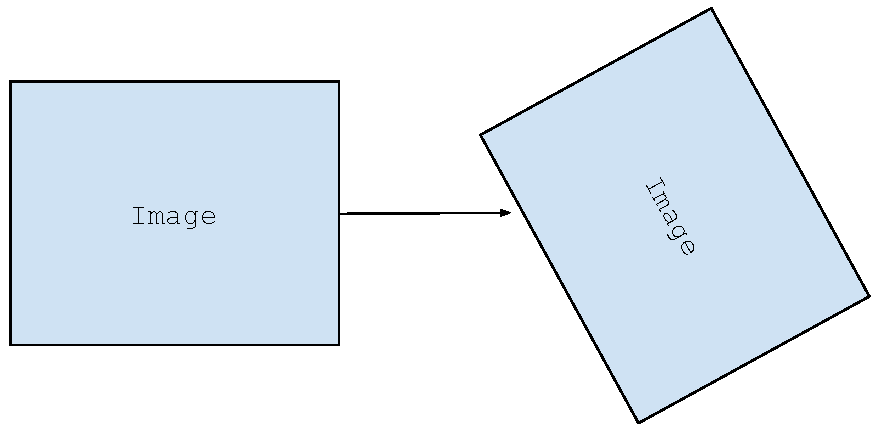
\includegraphics[width=\textwidth]{Chapter1/lit-review-img/rotation.pdf}
          \caption{Image rotation about the origin.}
          \label{fig:rotation}
      \end{subfigure}
      ~ %add desired spacing between images, e. g. ~, \quad, \qquad, \hfill etc.
      %(or a blank line to force the subfigure onto a new line)

      \begin{subfigure}[b]{0.45\textwidth}
          \centering
        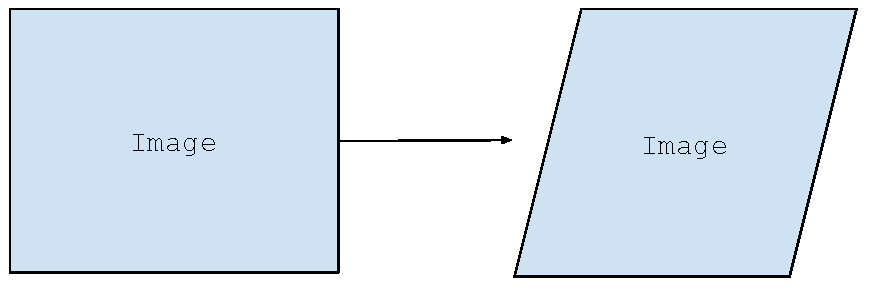
\includegraphics[width=\textwidth]{Chapter1/lit-review-img/xshear.pdf}
        \caption{Image shear in the $x$ axis.}
        \label{fig:x-shear}
      \end{subfigure} \hfill
      \begin{subfigure}[b]{0.45\textwidth}
          \centering
        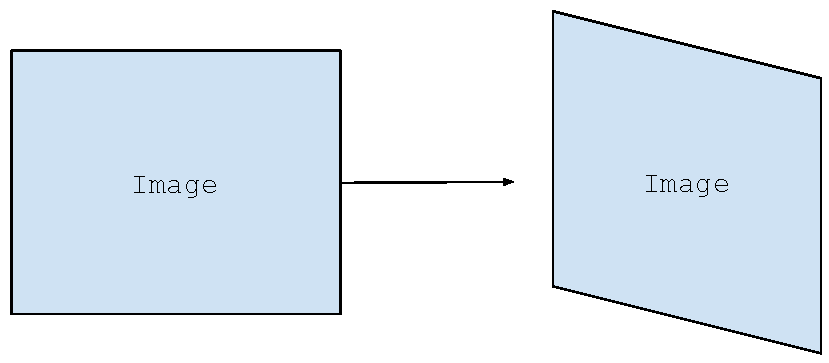
\includegraphics[width=\textwidth]{Chapter1/lit-review-img/yshear.pdf}
        \caption{Image shear in the $y$ axis.}
        \label{fig:y-shear}
      \end{subfigure}

      \begin{subfigure}[b]{\textwidth}
        \centering
        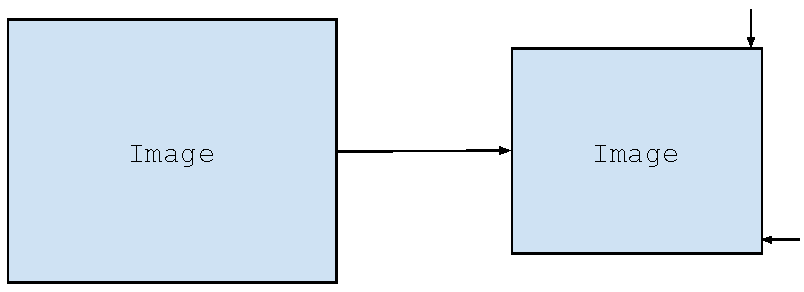
\includegraphics[width=0.45\textwidth]{Chapter1/lit-review-img/scale.pdf}
        \caption{Image scale in the $x$ \& $y$ axes.}
        \label{fig:scale}
      \end{subfigure}
    \caption{Image transformations executed by the \Gls{Congealing} algorithm}
    \label{fig:image-transformations}
  \end{figure}
\end{center}

\vspace{-1cm}

The entropy is calculated by assessing each individual set of pixel-locations in the `Pixel Stack' (see Figure \ref{fig:pixel-stack}), and by calculating the entropy of the empirical distribution of values in the Pixel Stack.

\begin{figure}[H]
  \center
  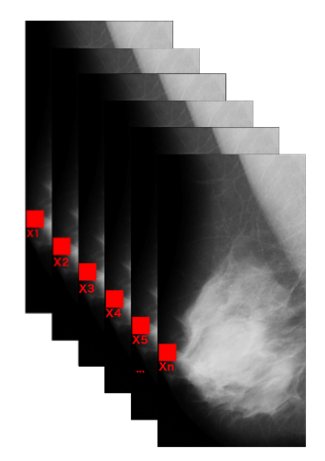
\includegraphics[scale=0.5]{Chapter1/lit-review-img/pixels.png}
  \caption{Each pixel from the same location throughout the set creates a `Pixel Stack'}
  \label{fig:pixel-stack}
\end{figure}

\subsubsection{Least squares Congealing for unsupervised alignment of images}

Further work was done upon the \Gls{Congealing} algorithm proposed by Learned-Miller by Cox et al. in 2008 \cite{Cox_Sridharan_Lucey_Cohn_2008}. They set out to address any performance issues and to remove the need for a pre-defined step size. It proposes to mitigate these issues by implementing an alternative method for aligning the images - utilising the Lucas \& Kanade algorithm for aligning a single image to another using a gradient descent approach \cite{Lucas_Kanade_1981}.

\subsubsection{Unsupervised Joint Alignment of Complex Images}

Huang and a team (notably including Learned-Miller) further extended the \Gls{Congealing} algorithm to be usable upon complex images - such as faces and cars at different orientations \cite{Huang_Jain_Learned-Miller_2007}.

This method removes the need to hand-label the input data and improves the performance of face recognition systems, by ensuring the objects are properly oriented prior to recognition.

\subsection{Image Alignment using Fuzzy Entropy}

Research has been undertaken in the past to investigate image alignment using fuzzy entropy metrics, however typically they were found to be computationally costly, and therefore slow to run on a conventional PC or laptop. This project will be investigating whether there are simpler, more light-weight fuzzy entropy metrics which could be implemented, for more everyday use in image alignment. It will also be investigated if, and further how, the outputs of these alignments differ per each fuzzy entropy metric.

Some of this work which has implemented a more computationally-costly \Gls{Congealing} algorithm is that presented by Mac Parthal\'ain and Strange in their 2013 paper \say{Fuzzy-entropy based image congealing} \cite{Mac_Parthalain_Strange_2013}.  Their implementation included dynamically-calculated fuzzy sets and a fuzzy similiarity relation matrix - allowing a comparison of all the objects to each other.
